\section{Discussion on the original paper}
\label{sec:discussion}
ADOP\cite{ruckert2022adop} is overall an excellent paper. It does not bring so much novel ideas but makes a considerable engineering effort to apply the core idea of NPBG \cite{Aliev2020} to large real scenes.
We'll discuss two main limitations of the paper in the next section.\\
\noindent \textbf{~\ref{subsec:limits_real_scenes}{: Real scenes $\approx$ biased evaluation}}. Evaluation on real scenes from the Tanks and Temple dataset \cite{Knapitsch2017TanksAndTemples} mixes two things:
\begin{itemize}
    \item the inherent neural rendering method (point based rendering) quality assesment.
    \item all improvements made by taking into account the camera pipeline.
\end{itemize}
Despite ablation studies to see the effect taking the camera photo pipline into account, the comparison to other methods is unfair and I'll propose a few ideas for a new benchmark to evaluate neural rendering quality in a more controlled environment for research purpose.\\
\noindent \textbf{~\ref{subsec:view_dependant_materials}{ : Inherent limitations to model view dependant material appearance}}. By construction, the ADOP pipeline does not have the ability to model view dependent effects such as specularities or reflections.

Finally, in section ~\ref{subsec:improvement_ideas}, I will discuss some improvement ideas I had while working on the re-implementation of the ADOP paper.

\subsection{Limitation: Benchmarking only on real scenes}
\label{subsec:limits_real_scenes}
\noindent \textbf{Focusing only on real scenes.}
Suprisingly, the authors do not mention any attempts to apply their method to synthetic scenes, like the NERF paper initially did and they mention that training a new scene requires a large amount of compute. This could mean they developped their method progressively on a few toy examples and didn't bother releasing results of these tiny examples. Or their method may simply not perform too well on synthetic scenes... which may include a lot of specular materials. Classical NERF test samples scenes usually contain a lot of specular materials where the rendering would most probably fail. I still think it would be beneficial to have a few synthetic scenes to test on including to make quick tests without the need of A100 40Gb trained for several hours.
On the other hand, since the main method's contribution are refining pose estimation (requiring the approximate differentiable aspect of the renderer) and the camera photo simulator, it's not surprising that they'd work on natural photos rather than simulation. 

\noindent \textbf{Camera pipeline module.}
The attempt of the authors to model the camera pipeline comes from a good intention. By including the camera pipeline as part of their rendering, they are able to: 
\begin{itemize}
    \item work in a linear color space where... performing additions or convolutions is equivalent to the real world.
    \item compensate exposure and colors shifts per scene.
    \item get a better accuracy on the Tanks and Temple benchmark which has a lot of exposure changes.
\end{itemize}.
I think they picked the low hanging fruits here: take care of most exposure changes to end up improving the metrics on the available benchmark: Table 4. from their paper shows that ADOP is better by a large margin than all other algorithms (except the M60 tanks scene which has been shot in manual frozen exposure). 
They didn't backport their idea to the comcurrent methods they compare to so I don't think the comparison is really fair (the point based method may simply not be the key element leading to good results).

Anyway, their claim to handle the camera imaging pipeline properly and adapt to it is legitimate, well crafted and justified in the paper. But it has a major caveat: results may crumble in case of a more complex or different camera ISP \footnote{Image Signal Processor} than the one from Sony A7SII or DJI X5R.
Please refer to ~\cref*{fig:ISP}

\begin{figure*}[h]
    \centering
    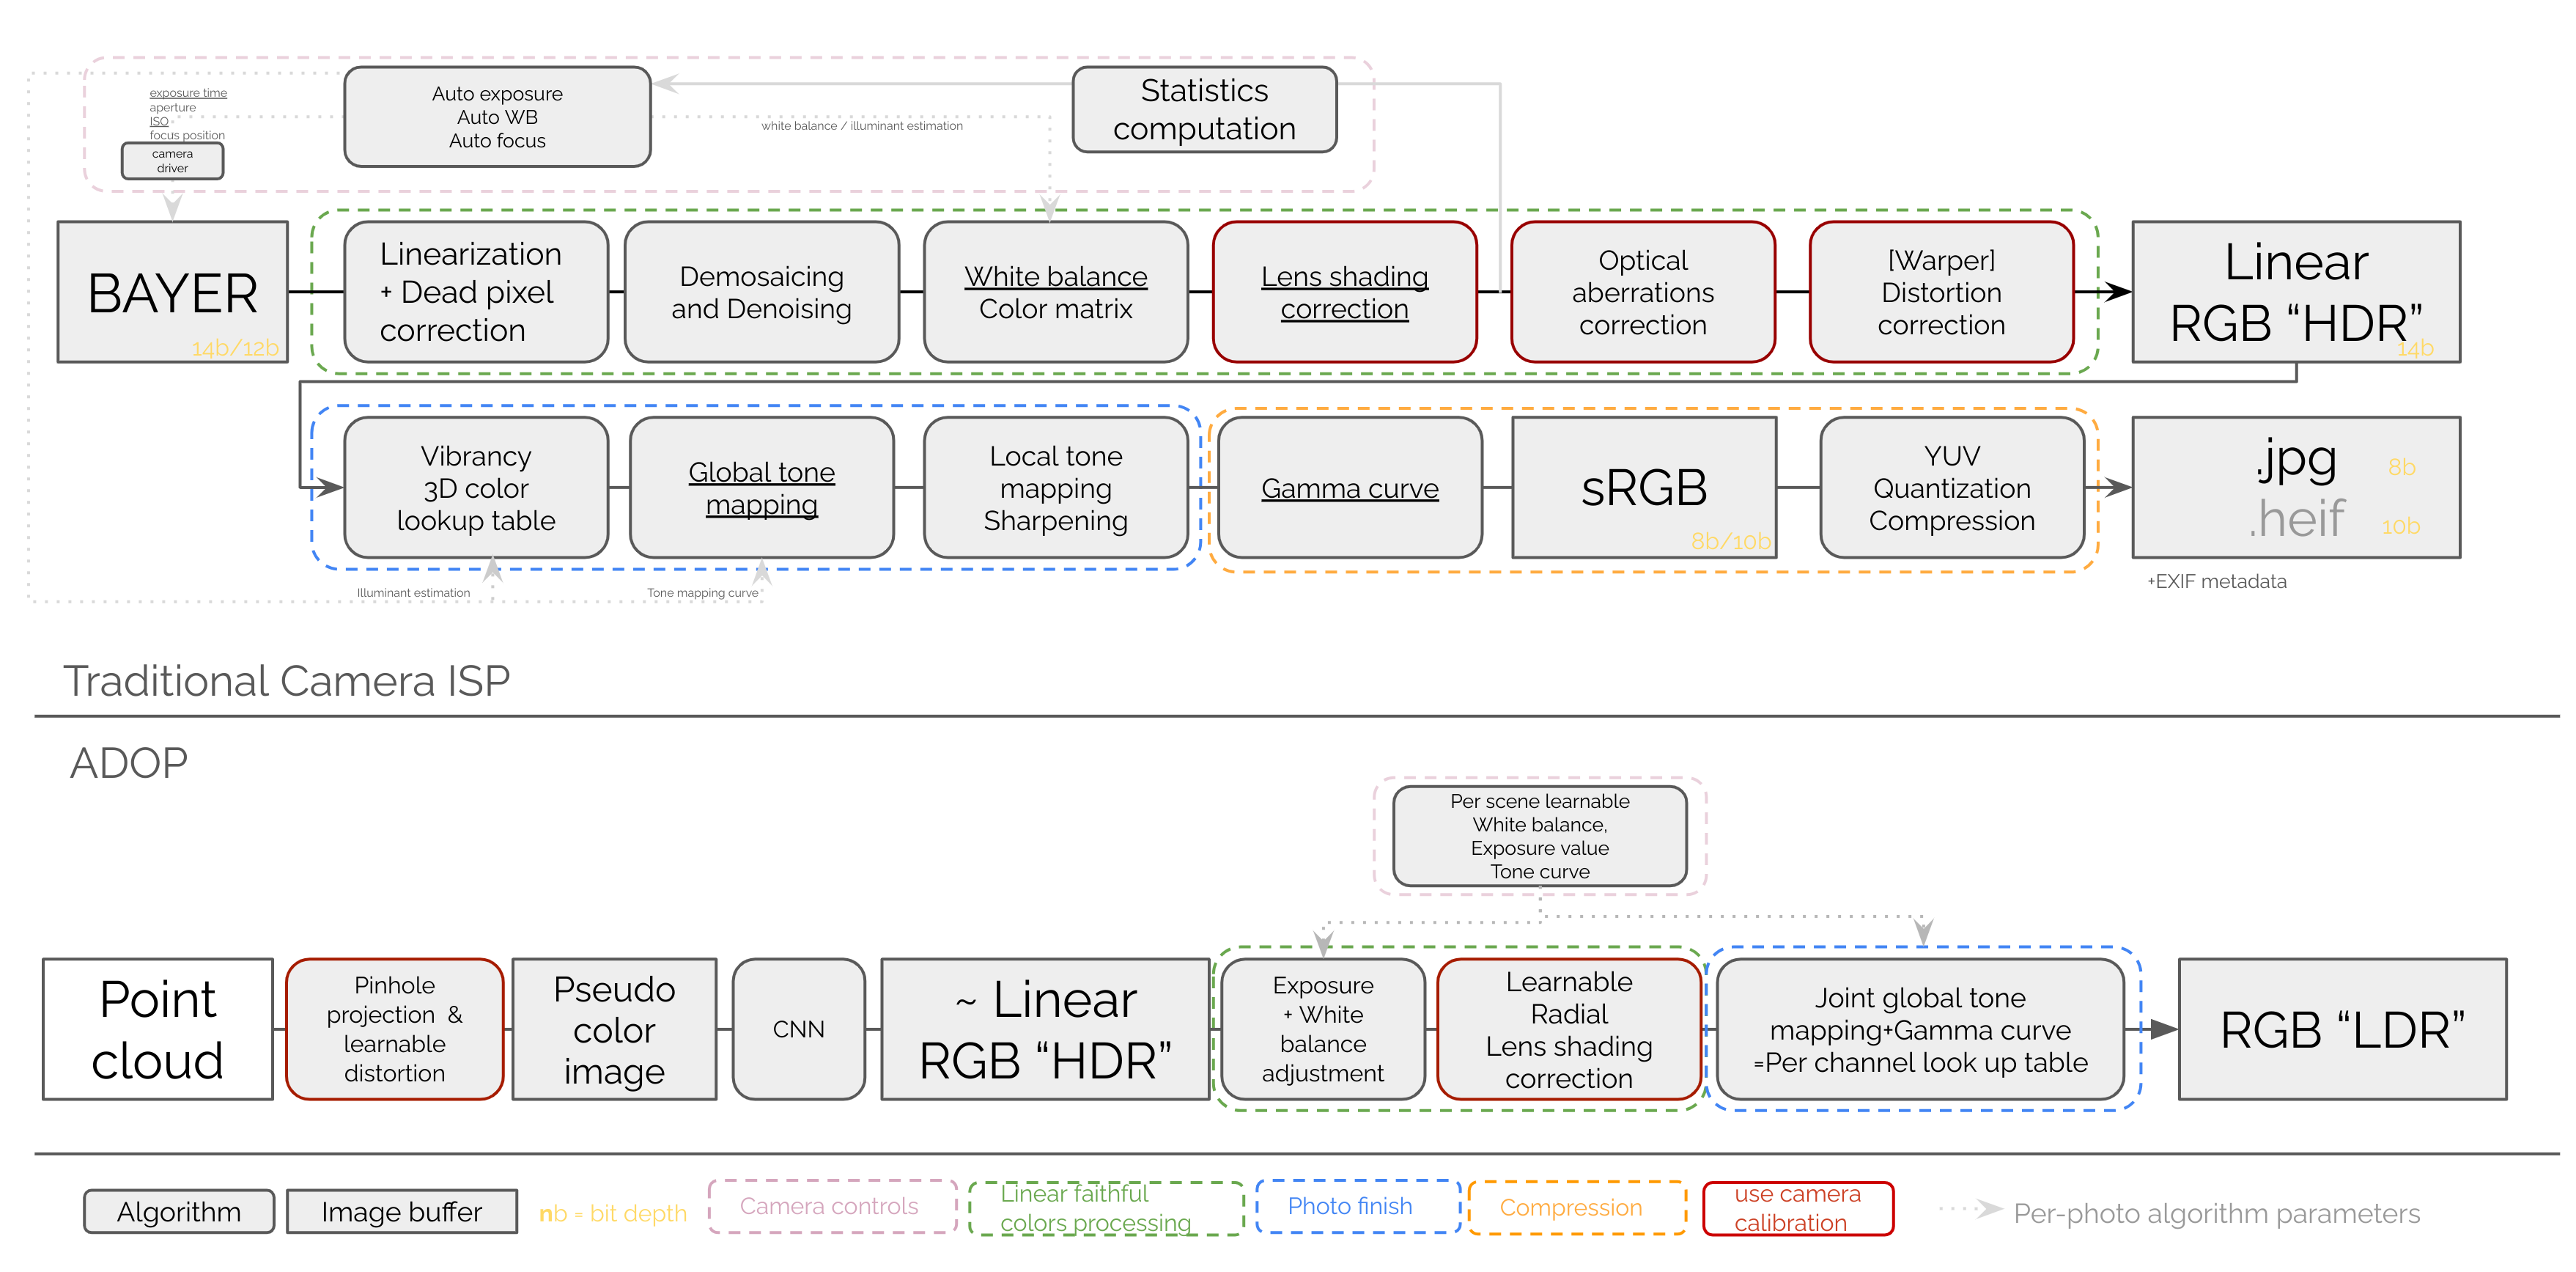
\includegraphics[width=0.9\textwidth]{figures/isp_pipeline_VS_ADOP.png}
    \caption{Comparing a modern ISP camera pipeline at the top versus the ADOP pipeline at the bottom which includes some learnable parameters such as the tone mapping curve, exposure compensation or white balance adjustments.}
    \label{fig:ISP}
\end{figure*}

Ablation study from the authors (table 3 and figure 6 of \cite{ruckert2022adop}) shows that ADOP results get better when including the camera module in the pipeline. problem is that we don't really know the exact impact of compensating the camera photo pipeline on the final result, at least compared to a scene imaged with perfect ideal linear HDR camera. 

If we carefully look at the Tanks and Temples dataset \cite{Knapitsch2017TanksAndTemples}, pictures are frames extracted from a mp4 video from 2 different high end cameras, sometimes using auto-exposure. Although it's a good initiative for researchers to keep on using fixed established benchmarks, Tanks and Temples was initially designed for 3D reconstructions (e.g. evaluate performances of Structure from motion like COLMAP estimation compared to a groundtruth lidar captured point cloud) rather than novel view synthesis. The idea is interesting but it will most probably fail with a modern smartphone camera which use local tone mappers and sometimes adapt colors locally. For instance, they're able to get a sky with cyan shift which looks like the camera picture (they fit the tone mapper correctly). Modern smartphone ISPs manufacturers have worked on this "cyan cast" problem (compress blue highlights instead of clipping when applying white balance) so compensating these algorithms will become harder and harder as they get more and more sophisticated.


\begin{figure}[H]
    \centering
    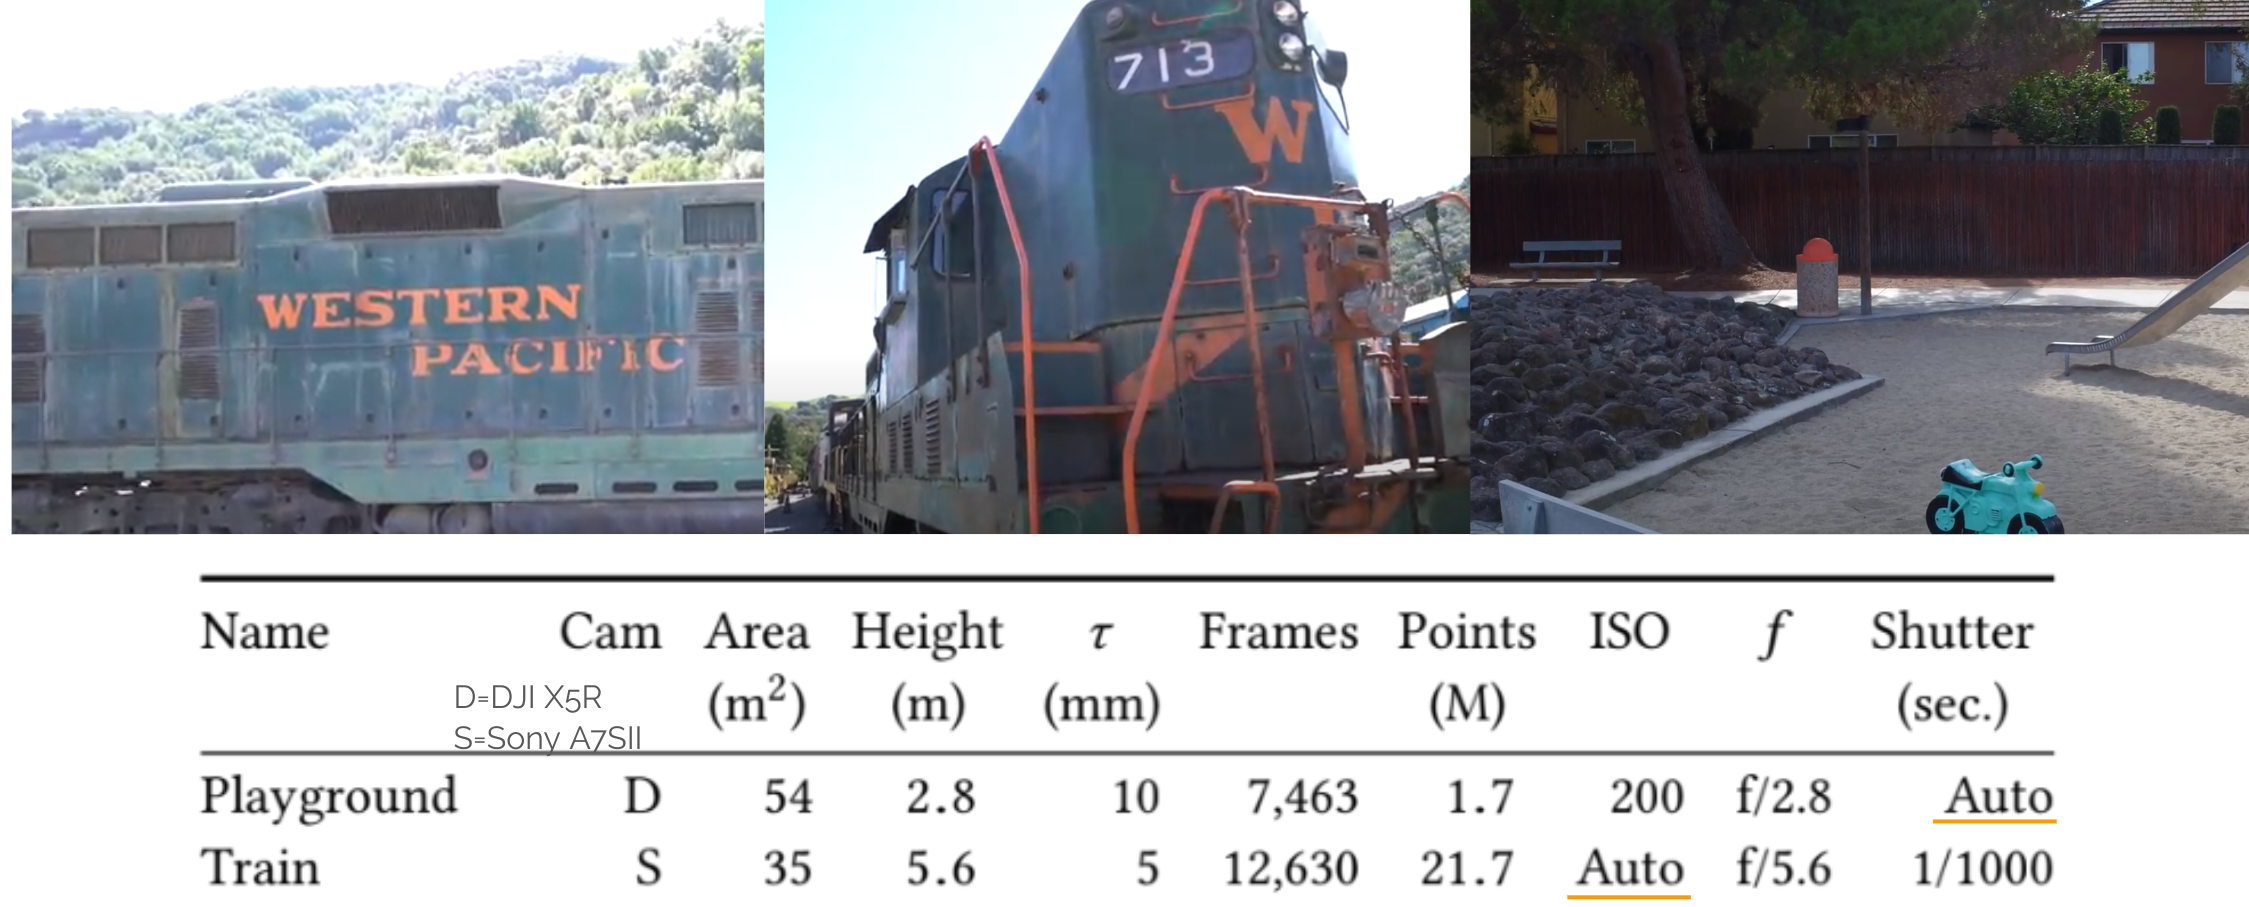
\includegraphics[width=0.45\textwidth]{figures/tanks_and_temples.png}
    \caption{Information on the scenes captured for the Tanks and Temples dataset with high end video cameras in addition to a Lidar point cloud. On the left, the "train" scene shows clear signs of overexposure. The playground scene on the right has an overall correct and steady exposure}
    \label{fig:tank_and_temples}
\end{figure}


\noindent Regarding my simplified implementation, I did not try to include the camera pipeline module not only because of limited time but also because simulating a realistic camera pipeline is a very difficult task.
For calibrated scenes, to mimick a realistic camera pipeline, one would have to:
\begin{itemize}
    \item output HDR linear images out of Blender (\textit{BlenderProc does not even offer EXR outputs at the moment}).
    \item mimick RAW files: inverse the blue "linear" blocks of figure ~\cref*{fig:ISP}. The idea of reversing the ISP has been proposed in \cite{brooks2018unprocessing}: apply inverse white balance and color matrices from typical values, mosaick, add realistic poisson+gaussian noise depending on sensor characteristics and ISO value...
    \item Mimick the ISP which goes from 12bit linear RAW bayer data to a 8 bit jpg (which is an extremely difficult task).
\end{itemize}
This is definitely \textbf{not a simplification} and I'll come to the conclusion that generally speaking, performing all evaluations in the linear domain is the best way to go and that novel view synthesis benchmarking would strongly benefit from an "upgrade":a sort of Linear Tanks and Temples carefully crafted by taking RAW shots with a high end DSLR.

\noindent \textbf{Switching to RAW format?} 
One of the potential way of creating a new benchmark would be to capture the scenes with a DSLR (like a full frame sensor) shot both in RAW and jpg (usually available on most cameras). RAW files would be post-processed by Adobe LightRoom or DxO Photolab with a neutral rendering: no tone mapping and neutral color rendering to get a Linear RGB set of images without any image compression. In case the sensor 12 or 14bits dynamic range is not sufficient, HDR captures could be achieved by bracketing. Intuitively, it sounds natural to use a tripod and merge the LDR linear images into a HDR linear image. But even handheld, all raw captures at various exposures could be used (let the alignment of bracketing images be implicitly done without any explicit need to merge exposures). These HDR images may serve as the ground truth for validation.

The main caveat of using RAW images is that there'll always be noise present proper to the camera sensor in the raw files. Since you get multiple views of the same scene, we can use the key concept proposed in Noise2Noise \cite{lehtinen2018noise2noise} that a neural network can be trained to denoise images without a ground truth images (it requires noisy burst of the same image instead). Here we have access to the same scene under different angles. The engine to implicity align them and get the right supervision is the rendering of the point cloud itself! The idea of using NERF to work on RAW data has been proposed in "NERFs in the dark" \cite{mildenhall2022rawnerf}.


RGB (raw demosaicked) linear format is the only space in which an evaluation of the rendering quality does not depend on the camera ISP.
If one would really like to check the effect Training images could be either the jpgs or the reprocessed RAW files using a more scenic rendering: vibrancy to make some colors slightly more saturated (e.g. blue for skies but avoid saturating red too much for skin tones), tone mapping (global or local), sharpening / micro contrast.

\subsection{Inherent limitations to model view dependant material appearance}
\label{subsec:view_dependant_materials}

\subsection{Improvement ideas}
\label{subsec:improvement_ideas}
A lot of my implementation work has been based on applying the ADOP paper to synthetic scenes.